\section{Proof-of-Concept Attack}
\label{sec:poc.attack}

\subsection{Testbed Setup}
\label{sec:attack.setup}

As a simple proof of concept, we wanted to perform a man-in-the-middle attack.
Since we don't have access to specialized router that supports packet eavesdropping
and manipulation, we used \texttt{scapy} to emulate router on a regular Ubuntu server.

\begin{figure}[ht]
    \centering
    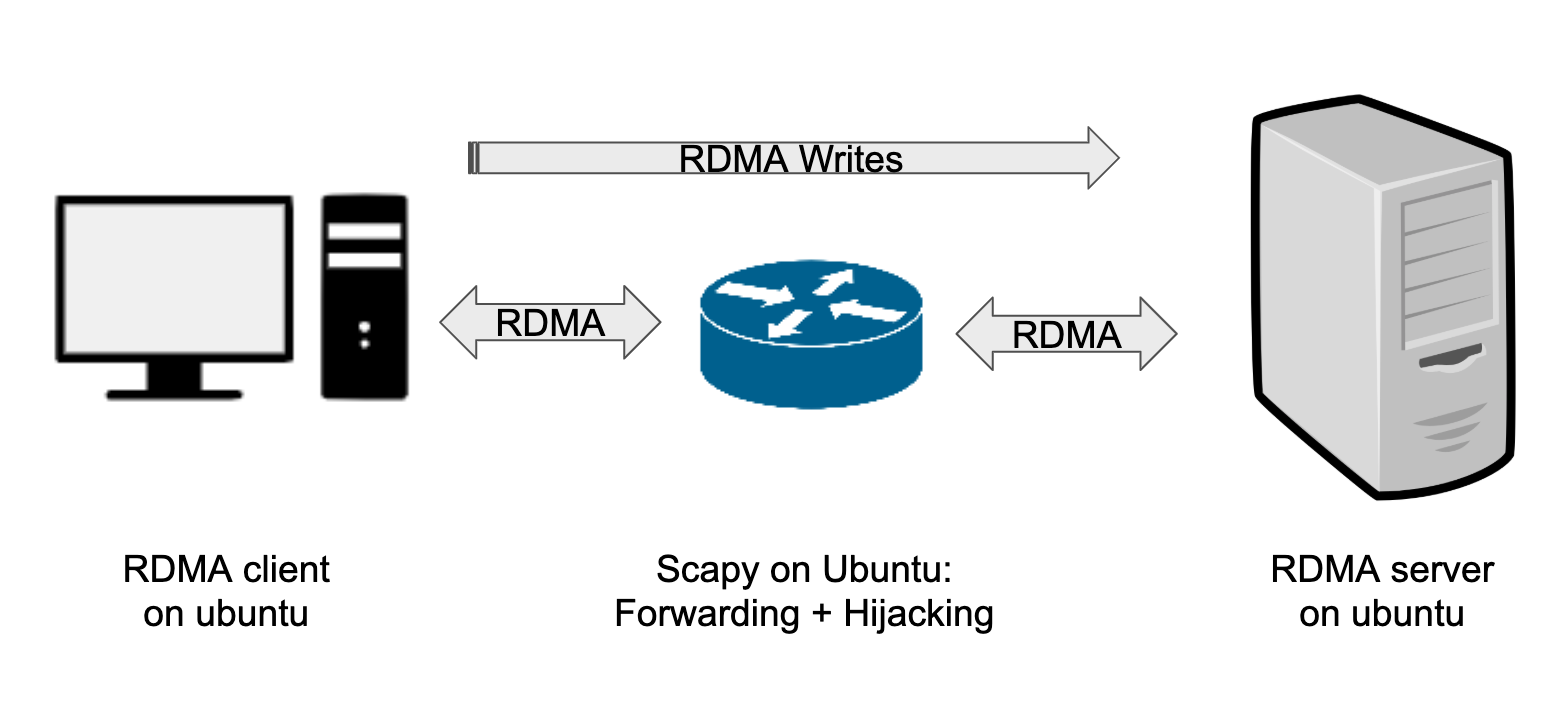
\includegraphics[width=0.5\textwidth - 5pt]{fig/attack_setup}
    \caption{Attack Testbed Setup}
    \label{fig:attack.setup}
\end{figure}

As show in \autoref{fig:attack.setup}, we run regular RDMA client and server
on two Ubuntu servers. Both machines are connected to the machine in the middle,
which uses \texttt{scapy} to sniff all \texttt{RoCEv2} packets, re-write the MAC
addresses and forward it to the other port. In the case of attackers present, we
allow the attacker to modify the packet as needed, after which we'll re-compute
the \texttt{RoCEv2} checksum according to the IBTA specs \cite{infiniband:iba.spec.vol1.v1.3},
RoCE annex \cite{infiniband:iba.spec.annex.roce} and RoCEv2 annex \cite{infiniband:iba.spec.annex.rocev2}.

We set up the \texttt{arp} entries manually such that both client and server think
they are talking to the each other directly, but in reality, the packets will all
go through the middle machine.

\texttt{scapy} is a \texttt{Python} module that allows packet sniffing, manipulation, injection, etc.
It internally calls \texttt{tcpdump} and works on raw socket as well, which gives us the ability to
re-write Ethernet-layer MAC addresses.

\subsection{Attack Model}
\label{sec:attack.model}

For the proof-of-concept attack, we choose to hijack the write address of RDMA write requests.

\begin{figure}[h]
    \centering
    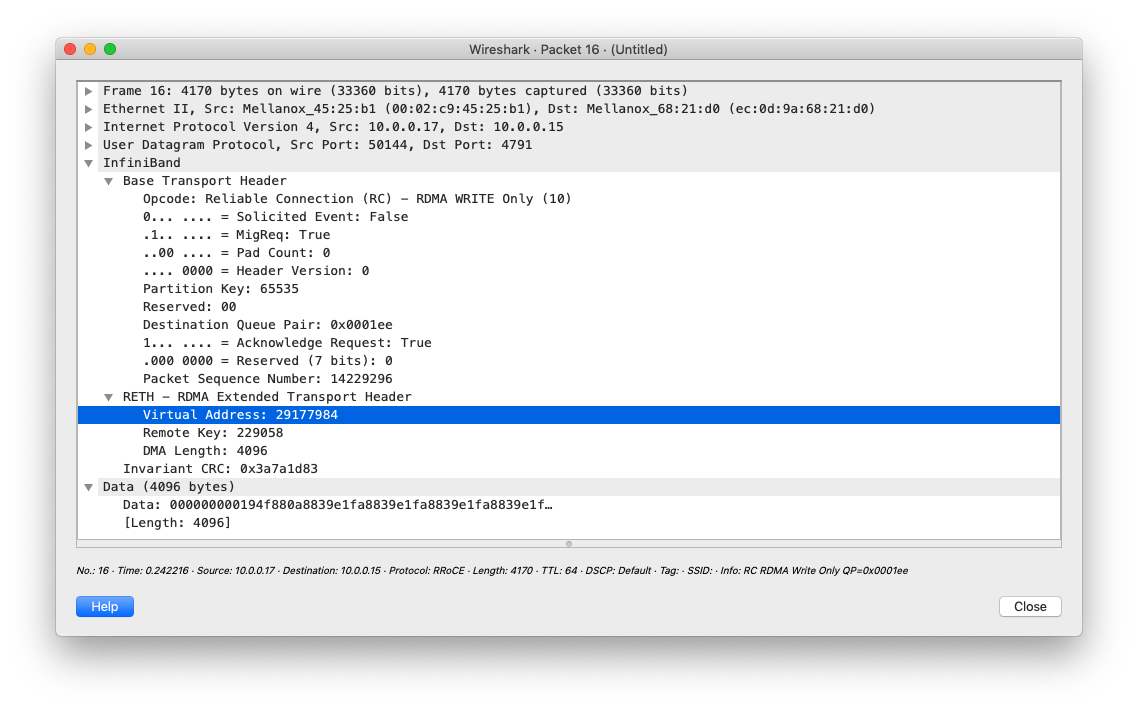
\includegraphics[width=0.5\textwidth - 5pt]{fig/rdma_write_packet_wireshark}
    \caption{RDMA Write Packet in Wireshark}
    \label{fig:attack.rdma_write_packet}
\end{figure}

RDMA WRITE allows the requestor/client to write data to the address space of the target application
on the target machine / server, using a remote key negotiated via prior authentication. However,
neither the key nor the virtual address is encrypted, as show in \autoref{fig:attack.rdma_write_packet}.

We decided to hijack all writes to the same address, which can be handy to carry out Throwhammer attack
as previously shown \cite{216055}.
For our PoC, our adversary remembers the virtual address of the first WRITE it sees,
and changes addresses of all subsequent WRITEs to be the same.

\subsection{RDMA Client/Server}
\label{sec:attack.rdma_app}

For simplicity, our RDMA client will issue $n$ RDMA WRITE requests after initial handshake and
information exchange needed for one-sided RDMA operations like RDMA WRITE. According to the attack model
described in \autoref{sec:attack.model}, our attacker hijacks all subsequent RDMA WRITEs. Thus, we compare:
1) client issues on RDMA write, and 2) client issues two RDMA writes to two different address.

We used a modified RDMA performance benchmark tool, which in the first case, issues one RDMA WRITE of 16 bytes,
and the second case, issues two consecutive RDMA WRITEs of 16 bytes each. At the end, both client and server
computes the SHA1 checksum of the buffer region. If the SHA1 digest matches, then it means all data have been
transferred successfully and not been tampered with.

\begin{table*}[ht]
    \begin{tabular}{c|c|c}
        Experiment \# & $1$ & $2$ \\ \hline
        SHA1 digest (client) & 609f05f73fb251aec1c7d8b25b4cbe1d2d1a1661 & b262a891b5dfc43930d6aa733e9741e625126a89 \\
        SHA1 digest (client) & 609f05f73fb251aec1c7d8b25b4cbe1d2d1a1661 & 2488224f4d0dff339e01d1694a0bee162eb8c358 \\
    \end{tabular}
    \caption{RDMA Proof-of-Concept Result}
    \label{table:attack.result}
\end{table*}

As show in \autoref{table:attack.result}, in the first case, there is only one RDMA WRITE, so the attacker doesn't
modify the requests at all, thus the SHA1 digests match. But in the second case, since there are two RDMA writes, the
second RDMA WRITE is hijacked so the buffer for the second WRITE wasn't wrote successfully. Thus the SHA1 digests
don't match. This simple proof-of-concept shows that it is (very) possible for attackers who compromised a switch to
carry out RDMA attacks like Throwhammer and more.

\subsection{Result}
\label{sec:attack.result}
